\documentclass[12pt]{amsart}
                   

\usepackage {mathpartir}
\usepackage{bcprules}
%\usepackage{listings}
                       
\usepackage{graphicx} 
\usepackage[left=2.5cm, right=2.5cm,top=2.5cm,bottom=2.5cm,nohead,nofoot]{geometry}   

\include{myPreamble}
\include{lgmheader}     

\ifpdf
\usepackage[pdftex]{graphicx}
\else
\usepackage{graphicx}
\fi

\ifpdf
\usepackage{pdfsync}
\if


\title{Brief Article}
\author{David F. Snyder}

%\address{Dept. of Math., Texas State University--San Marcos, San Marcos, TX 78666}



\begin{document}

%\maketitle
 
\section{Introduction}\label{sec:introduction} % (fold)
   Knot and link tabulation continues to be a lively area of scientific research and promises to be useful to areas of science such as quantum computing and DNA unpacking [citation].  The past 20 years have seen major advances in knot classification, the development of knot invariants, and computational methods for tabulating knots and links.  Currently there are tables of all prime knots and links of up to 23 crossings [citation]. While current algorithms provide complete tables of knots, winnowing these tables of duplicates is a time consuming task. Moreover, as knot tables have proved of use to researchers in genetics, and may prove to be to researchers in quantum computation, the need to search these tables in meaningful ways presents itself. For example, of the 4,976,016,485 prime, non-oriented, alternating knots with minimal crossing number of 22, which are slice knots?  Of course, knot invariants are used to distinguish knots. The activity here will develop the newly found strong knot invariant of Meredith and Snyder [citation], investigating further characteristics of the knot encoding. In addition, based upon these characteristics, the PI and co-PI will develop a query language for knot theorists capable of efficiently coaxing and prodding mathematically useful information from tables of knots and links. The possibility of using this new knot invariant to make current algorithms more efficient and effective will be investigated as well. In particular, a knot server will be deployed based upon current web standards (XML and XQuery) and spatial logic modelers. One graduate student and a team of 2-3 highly talented high school students will round out the team.
This narrative first gives a brief overview of knot notation systems and of software for knots studies. Then a summary of the π-Calculus and spatial logics is provided. The succeeding section then ties the previous two sections together: a description of the Meredith-Snyder knot encoding and its properties. The next section gives the specifications for the promised knot server. The final sections discuss broader impacts, significance, and the educational component.
% section introduction (end)

\section{A brief overview of relevant knot notation systems}\label{sec:notation} % (fold)
A brief overview of relevant knot notation systems
The knot notation systems we focus upon herein are the Gauss Code, the Dowker-Thistlethwaite (DT) Code, the Conway Code, and the Master Code of Rankin, Schermann and Smith. Other notation and naming systems exist but don’t pertain directly to the proposal.
• Gauss used regular knot projection to arrive at what is now called the Gauss Code of a knot. The Gauss code is the first knot notation system. In 1847, J.B. Listing classified knots up to 5 crossings by analyzing knot projections. P. G. Tait used an encoding he used in the 1870’s to classify knots up to 7 crossings. This encoding is an extension to the Gauss Code. One begins somewhere on the knot projection, proceeds along the knot applying labels to the first, third, fifth etc. crossing until all crossings are labeled; then one traverses the knot once more, writing the label of each crossing in the order that you reach it, attaching a plus or minus sign, depending on whether you are crossing over or under. 
• Using Kirkman’s classification of certain polygons, Tait (and Little, using similar methods) was able to tabulate knots up to 11 crossings. Tait’s system included using a simple reduction rewrite strategy within his notation system. 
• Reidemeister developed a reduction rewrite system for knot projections (“the three Reidemeister moves”).
• Conway developed a clever notational system for tangles, finding an algebraic-like system for tangles (the tangle calculus) that led to several methods of reduction rewrites. He used this system to tabulate knots and links of 11 crossings by hand, in one afternoon (an effort that took Tait and Little years of work), discovering one omission and a few duplications in the process. Conway’s system can be used to classify all arithmetic (also called algebraic, or rational) knots. The Conway code for a knot originally was given as a “basic polyhedron” followed by a sorted list of arithmetic tangles. See Conway’s paper for details. This system has extensions by Caudron and by Bangert.
• Dowker created a variation of Tait’s notational system that is easier to implement computationally. Dowker and Thistlethwaite made it the basis for an algorithm that successfully enumerating knots of up to 13 crossings. Not every DT code is valid, i.e. an arbitrary DT code may not correspond to an actual knot, and two distinct composite knots may share the same DT Code [citation Scharein’s thesis]. However, a valid DT code for a prime knot specifies the knot uniquely. In their paper, Dowker and Thistlethwaite develop an algorithm to filter out invalid cases. They also give a reduction system to remove duplicates from their enumeration.
• Calvo developed an inductive algorithm, thereby sidestepping the need to check validity of DT codes. However, duplication then becomes a larger issue. Calvo had the insight that understanding the deeper flype structure of prime, non-alternating diagram led to greater efficiencies in his algorithm. The Calvo algorithm was essentially refined in the development of a notational system due to Rankin, Flint, and Schermann [citation], based on what they call the group code which reminds one of the Gauss code, but using a Conway-like insertion scheme to allow for easy reduction of flype structures in the notation.
Desirable properties for a knot notation system
Due to complexity considerations, one may well despair of a knot notation system that would allow for classification of all knots. However, in designing a notation system, from the history of knot tabulation and classification we can gather that the following properties of the notation system would be eminently desirable:
• Each code in the notation should represent a knot (or if this is not the case, those codes that do not represent a knot should be quickly recognizable).
• The notation should have a calculus with which to reduce and simplify encodings. Each step of simplification or reduction should result in an encoding representing a knot isotopy equivalent to the originating knot.
• The notation system should have the theorem: The encoding in the notation of a given knot can be reduced to a (finite non-empty set of equivalent) minimal encoding(s).
• Another desirable theorem: If a knot has two (or more) minimal reduced encodings, these encodings are transparently equivalent notations for a knot isotopy-equivalent to the original.
• Important desirable corollary of the previous theorem: Two knots that have equivalent minimal reduced encodings are isotopy equivalent.
• Another desirable theorem: The notation can be used to classify a class X of knots, where X contains a previously classified class of knots (for example, arithmetic knots (also know as algebraic knots) and bracelets) but is not previously classified itself.
• There will be a formal language in which to describe properties and invariants of notation objects that reflect interesting properties of knots. This language should also be useful in selecting specific sets of knots (such as the set of all 21-crossing prime alternating links containing the tangle 3/4). This language ideally should be scaleable and be applicable to tables of indefinite size.
% section notation (end)

\section{A brief overview of knot software}\label{sec:a_brief_overview_of_knot_software} % (fold)
This is a brief overview of knot software, to illustrate the relevance of this proposal. A general shortcoming in these tables is that one cannot search the tables based on a particular criterion, such as “Give me all the genus 7 knots having minimal crossing number between 15 and 17.”
The online Table of Knot Invariants [citation] lets the user choose one of the knot tables (or subtables) for knots of 12 or fewer crossings and choose from a wide variety of invariants and notations that they wish to see. The resulting table is given with the desired invariants and notations listed for each knot.
The online KnotAtlas [citation] contains Mathematica® code (the package KnotTheory [citation]) and a visual database of knots and links up to 11 crossings.
Rob Scharein’s KnotPlot [web citation, citation] is extensive and extensible software that has a multiplicity of capabilities. It contains a visual database, for example, of all knots up to 10 crossings. KnotPlot also supports tangle calculus and many other features. KnotPlot is open source software and can be used to generate knot representations suitable for import into the PIs’ software system. Scharein has built the Knot Server [web citation], which is intended to data and invariants of knots within the tables of KnotPlot, though at this writing the calculation of invariants is not functional.
N. Imafuji and M. Ochiai [citation] developed Knot2000 (K2K), a Mathematica®-based package that allows for extensive computation with knots and links. S. Jablan and R. Sazdanovic [citation] have used this package and their own webMathematica® code to develop the excellent on-line site LinKnot that introduces computational methods in knot tabulation and discusses other aspects of knot theory as well.
The website Knotilus [citation] of Rankin et al. has extensive tables of knots and links up to 23 crossings, with browsing of these tables possible via a known Gauss or Dowker-Thistlethwaite code, or via a classification scheme, with a java-based applet for displaying (and drawing) knots.
Gruber [citation] has posted online tables of rational knots of up to 16 crossings, though some errors in the tables exist, only a few invariants are calculated, and the tables are not searchable.
% section a_brief_overview_of_knot_software (end)

\section{Concurrent process calculi and spatial logics }\label{sec:concurrent_process_calculi_and_spatial_logics_} % (fold)
In the last thirty years the process calculi have matured into a remarkably powerful analytic tool for reasoning about concurrent and distributed systems. Process-calculus-based algebraic specification of processes began with Milner's Calculus for Communicating Systems (CCS) [53] and Hoare's Communicating Sequential Processes (CSP) [41], and continue through the development of the so-called mobile process calculi, e.g. Milner, Parrow and Walker's π-calculus [57, 58], Cardelli and Caires's spatial logic [17], or Meredith and Radestock's reflective calculi [50, 51]. The process-calculus-based algebraic specification of processes has expanded its scope of applicability to include the specification, analysis, simulation and execution of processes in domains such as:
• telecommunications, networking, security and application level protocols [1, 2, 12, 47];
• programming language semantics and design [12, 36, 37, 73, 75];
• webservices [12, 47, 48];
• and biological systems [16, 22, 61, 62].
Among the many reasons for the continued success of this approach are two central points. First, the process algebras provide a compositional approach to the specification, analysis and execution of concurrent and distributed systems. Owing to Milner's original insights into computation as interaction [54], the process calculi are so organized that the behavior – the semantics – of a system may be composed from the behavior of its components [35]. This means that specifications can be constructed in terms of components – without a global view of the system – and assembled into increasingly complete descriptions. The PIs in this project model knots as being concurrent and distributed systems of crossings. Thus, new computational models of specific classes of knots can be constructed and when they are, thanks to compositionality they can be assembled to extend notations for previous classes (e.g as Conway notation revealed the class of arithmetic knots). In this way, a coherent framework for extending knot notation systems exists. Moreover, there is an underlying mathematical structure in which to search an entirely new population of knot invariants – dynamic algebras.
The second central point is that process algebras have a potent proof principle, yielding a wide range of effective and novel proof techniques [59, 67, 68, 69]. In particular, bisimulation encapsulates an effective notion of process equivalence that has been used in applications as far-ranging as algorithmic games semantics [3] and the construction of model-checkers [13]. The essential notion can be stated in an intuitively recursive formulation: two processes, P and Q, are to be considered bisimilar, if whatever action can be observed of P, taking it to a new state P’, can be observed of Q, taking it to a new state Q’ such that P’ is bisimilar to Q’. Part of what makes this notion so robust and widely applicable is that it is parameterized in the actions observable of processes, P and Q, thus providing a framework for a broad range of equivalences and up-to techniques all governed by the same core principle [67, 68, 69].
% section concurrent_process_calculi_and_spatial_logics_ (end)
    
\section{Knots as processes}\label{sec:knots_as_processes} % (fold)

This section contains an overview of Meredith and Snyder’s approach [citation]. An n crossing knot K is modeled dynamically as a concurrent system of n+1 processes consisting of n crossing processes and one wiring process. The latter process can be thought of as the computational equivalent to Conway’s “basic polygon,” if the knot is in minimal crossing number form. Using the well-established symbolism of mobile process calculi, the process is represented abstractly as follows:  . The wiring process is composed of   concurrent wire processes that correspond to edges in the 4-valent graph of the knot shadow (so the wiring diagram can be constructed from the DT code of the knot projection). Thus the knot is represented as  , where   represents the natural extension of the binary operator  (called “Par”) to tuples of processes. The crossing and wire processes have further substructure. The substructure of crossings is now outlined (see [CKC citation] for a sketch of the wire process or [cite paper] for details on both).
\subsection{Basic interpretation}\label{sub:basic_interpretation} % (fold)
A crossing is conceived as a process having four possible behaviors, as shown in its formula and the corresponding diagram.
  \begin{figure}[tbp]
    \centering
    \scalebox{0.27}[0.270]{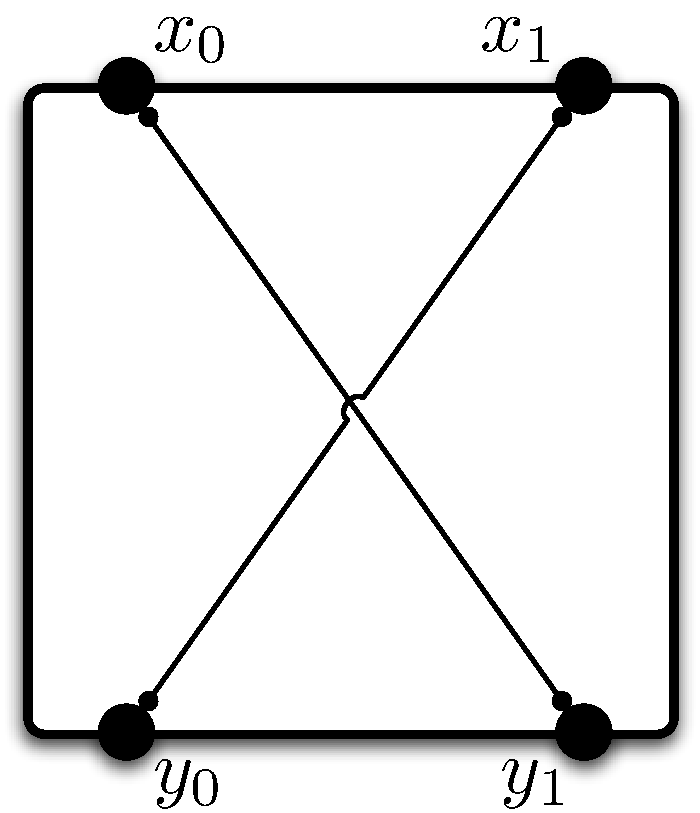
\includegraphics[viewport=0 0 390 360]{BasicCrossingCircuit.pdf}}
    %\caption{ here  }
\end{figure}
\begin{eqnarray}
  \lefteqn{ C(x_0,x_1,y_0,y_1,u) := } \nonumber \\
  & & x_1?(s).y_0!(s).(C(x_0,x_1,y_0,y_1,u)|u!) \nonumber \\
  & & + y_0?(s).x_1!(s).(C(x_0,x_1,y_0,y_1,u)|u!) \nonumber \\
  & & + x_0?(s).u?.y_1!(s).(C(x_0,x_1,y_0,y_1,u)) \nonumber \\
  & & + y_1?(s).u?.x_0!(s).(C(x_0,x_1,y_0,y_1,u)) \nonumber
\end{eqnarray}

 A crossing process has four ports $x_0,x_1,y_0,y_1$   and a hidden synchronizer $u$. Each port has a partner port, linked as shown in the diagram (note the relationship to Conway's $\pm 1$ tangles [citation]). For example, the first behavior (indicated by the first term of the summand) is that the process listens at port $x_1$   for a signal $s$  (which will come, if at all, via the wiring process). Having heard $s$, the signal is passed directly to the port $y_0$  where the signal is then broadcast via the wiring process. Then the process alerts the hidden synchronizer  that a signal has been passed between the ports, while concurrently preparing itself for further signal processing. The second summand represents a signal passing along the same strand in the opposite direction. The third and fourth summands are similar to the first two, except that before passing any received signal to its partner port, the process waits for a signal from the synchronizer $u$ before allowing the signal to pass. So the role of $u$ is that of a traffic controller who gives priority to traffic over the route between $x_1$ and $y_0$, mimicking an over-crossing.            
% subsection basic_interpretation (end)

\subsection{The syntax and semantics of the notation system}\label{sub:the_syntax_and_semantics_of_the_notation_system} % (fold)

Having found a way to encode knots as a synchronous concurrent process, then the tools of corresponding logical calculi become available. The approach is rooted in the spatial logic described in Caires [citation]. The process model (synchronous π-calculus) on which the logic is based is fundamental and of importance to future development of the knot notation being developed here, but the syntax and semantics of that logic receive the narrative focus. For now, know that there is a congruence relation   on the set of all processes in the model and that this structural congruence contains, for example, the relations that allow the inference that the collection is a commutative monoid under the operation Par. Let   denote the sub-collection of all processes that are knot encodings arising from a regular knot projection. The syntax and the semantics form the basis for constructing more meaningful and sophisticated queries of the knot tables than has been possible to this point. The following table shows a little of the syntax and semantics in this spatial logic. Here, the letters A and B are formulae that each represent a property a researcher may wish to query, while P, Q, and R are processes representing specific knots (up to ambient isotopy). This formulaic approach may also be used to automatize the culling of duplicates from a list generated by a knot tabulation algorithm.
 	(True)	 	 
 	(Negation)	 	 
 	(Conjunction)	 	 
 	(Void)	 	 
 	(Composition)

% subsection the_syntax_and_semantics_of_the_notation_system (end)   

\subsection{Characteristic formulae}\label{sub:characteristic_formulae} % (fold)

Of even more interest to knot theorists is the existence of characteristic formulae that provide (computationally decidable) characterization of processes up to a predetermined level, modulo a (decidable) extension of structural congruence. This provides an infinite sequence of characters, and thus an infinite sequence of knot families, to investigate, in the vein of what Conway intuited in his 1997 lecture at MSRI, entitled “Knotation” [citation]. For details of these characteristic formulae, see [citation, Caires, p.10]. Thus not only will the work proposed here provide computational methods for sophisticated queries of existing knot tables, a new field of knot characters and invariants to explore.
% subsection characteristic_formulae (end)   	 

\subsection{Example formulae}\label{sub:example_formulae_} % (fold)
                            
Two example formulas are given that demonstrate the powerful type of searches that current knot software cannot do. A reminder: the value of the work proposed here is not just powerful search mechanisms such as these, but also exploration of new knot characteristics. 

% subsection example_formulae_ (end)



% section knots_as_processes (end)

The proposed work and plan
Meredith and Snyder have established an encoding of knots into the π-calculus with the appealing property that two knots are ambient isotopic if and only if their encodings as processes are bisimilar [52]. Three principles derived from this work guide the investigation proposed here:
1. to extend the well-established paradigm of associating algebras to topological spaces to the setting where the algebras hosting such invariants have dynamics –  in the sense that they explicitly represent or embed a model of computation;
2. to exploit compositionality to expose those features of a space that may be analyzed locally (like the polarity of crossing in a knot diagram) versus those that require global information (like the orientation of a knot);
3. to establish a framework in which the proof principle and attendant proof methods of bisimulation may be exported to algebraic topology.
Another feature of the proposed line of research is that it makes essential use of mobility [54, 55, 56, 58, 67], that is the ability of processes to change their communication topology (the who-talks-to-whom graph) during the course of their execution. Up to this point, research in the connection between process algebras and topological spaces has dealt exclusively with non-mobile computations. This proposed encoding uses mobility to represent crossing information and exposes knot-orientation as essentially global information that must be spread throughout the specification.
The investigators have taken note that dual to the process calculi is a family of logics known as the Hennessy-Milner logics (HMLs) [35, 55]. Formulae of these logics typically denote sets of processes. To date, little has been done regarding the application of the HMLs to the connection between concurrency and topological theories [34, 40]. In addition to building on the work of Meredith and Snyder this grant will fund an exploration into using the HMLs, especially the subfamily of spatial logics [13, 14, 15], for searching repositories of known knots and braids. 
Spatial logics constitute a subfamily of the HMLs. They admit formulae to express both behavioral and topological aspects of processes [13, 14, 15]. Recently, it was recognized that model-checking HMLs, in general, and spatial logics, in particular, can be adapted to provide a powerful search mechanism [49].  Building on work establishing canonical ways to represent metabolic, signaling and transcription networks in the π-calculus [22, 61, 62], Biosimilarity LLC is already employing this method to build software tools for searching biological pathways. Employing the encoding of Meredith and Snyder [52] and working closely with Snyder, Biosimilarity LLC will extend their system to provide a webservice allowing researchers and students to search for knots in a repository on the basis of rich structural information and partial descriptions.
Work to be undertaken
The major part of the work will be the development of an online software system for experimental exploration of existing knot tables and of knot and braid invariants.
1. This component develops the avenue of investigation resulting from the Co-PI’s discovery of a faithful embedding of Knot Theory into the π-calculus [52] and the natural extension of this to Braid Theory.
2. Knot and braid theory are accessible entry points into research mathematics for the prepared undergraduate or bright high school student. The selected students will get some hands-on training in concurrent programming; they will be introduced to the π-calculus.
3. The approach will yield new knot and braid invariants.
4. Results of the overall team will be viewable online by the public.
Part of the work will also be wide-spread dissemination of results. This will be achieved in three ways.
1. Conferences, meetings, and workshops separately or jointly attended by PI (local, regional, national, and international), co-PI (Texas State, national, international), graduate student (local, regional, and national) and High School students (Siemens-Westinghouse).
2. Journal articles and other publications, by the PI, co-PI, and graduate student.
3. Web presence, in which the entire team participates.
General plan of work
The process by which the above objectives will be reached is now described.
The work will be carried out over a 2 year period. The project will begin 1 September 2007 and terminate on 31 August 2009. 
The second component will have a distributed nature for the majority of the project. The high school students will be attending Mathworks during summers, returning to their home campuses for the school year. Mathworks has experience with supporting faculty-student projects during the school year. Contact with students during the school year will be via e-mail and phone, and during competition heats. When these students are attending Mathworks, the PI (and post-secondary assistants) will meet daily with their student team regarding their actual research project and join them on scheduled weekend activities to build team identity. 
The third component of the work will involve mainly the PI and co-PI. They will exchange approximately week-long visits every quarter (July, October, January, April, and June) to collaborate more efficiently on this component. On these visits, they will also assess progress of team members and progress to the aim of each of the three components of the project. 
General personnel effort
The PI will be devoting 25\% of the academic year and 100\% (of two months) of each of the two summers to this project. The co-PI will be devoting 35\% of each year to the project; the co-PI will perform the majority of his work at his home site, Biosimilarity LLC in Seattle, and will visit the Texas State site once per quarter during the project. The co-PI will visit near the beginning of the project to interact with the students. The PI and co-PI have successfully worked together at-a-distance using a combination of e-mail, internet messaging, and internet telephony; they will continue to do so during this project as well, at least twice weekly.
A graduate student at the Master’s level from Mathematics, will be recruited or hired at the beginning of the project, with the aim that they come from an underrepresented group. The graduate assistant will be at 50% effort.
The high school students will attend MathWorks from late June to late July. The co-PI will come for an extended visit during this time to familiarize the Mathworks team with the process logics.
Equipment and materials
An 2-node Apple workgroup cluster is requested for the Texas State site and a 2-node cluster for the Biosimilarity site. The co-PI will be in charge of directing and managing the software development. The two nodes are needed for the co-PI to have the specific machine architecture envisioned for serving the knots and braids component, as well as the deeper investigation of simplicial complexes and homology in the π-calculus setting. Instructional materials for the students will be purchased as well.
Knots and Braids component
The aim of the knots and braids component is to provide a package somewhat similar to the knot server coming out of (http://www.colab.sfu.ca/KnotPlot/KnotServer/). The primary difference is that instead of providing search solely on the basis of crossing number and index, the search mechanism will offer a sophisticated query language based on spatial logic. Spatial logics constitute a subfamily of the HMLs. They admit formulae to express both behavioral and topological aspects of processes [13, 14, 15]. Recently, it was recognized that model-checking HMLs, in general, and spatial logics, in particular, can be adapted to provide a powerful search mechanism [49].  Building on work establishing canonical ways to represent metabolic, signaling and transcription networks in the π-calculus [16, 22, 61, 62], Biosimilarity LLC is already employing this method to build software tools for searching biological pathways. Employing the encoding of Meredith and Snyder [52] and working closely with Snyder, Biosimilarity LLC will extend their system to provide a webservice allowing researchers and students  (and the public-at-large) to search for knots in a repository on the basis of rich structural information and partial descriptions. See the figure on the previous page.
The work to extend the Biosimilarity system will be carried out primarily by the co-PI over the course of the first year. The bulk of the work will be to extend the existing system to support integration with the open source tool KnotPlot to generate knot representations and then import them into a process algebraic representation suitable for model-checking with a spatial logic model-checker. After this, the work will focus on usability, taking data from usage patterns and feedback from students and researchers using the system to improve usability, performance and robustness of the system.
Spatial logic component
The PI and co-PI will continue their investigation of representations for simplicial complexes in a reflective calculus with the aim of constructing one in which topologically equivalent complexes translate into observationally equivalent systems. This result would provide means of implementing a computationally efficient, verifiable method of spatial discrimination that does not rely on the traditional formulation of homology. Further investigation will be needed to reveal if such calculi can provide finer topological detail.
Background for the educational component
One Mathematics graduate student will participate in the project. Ethnic minorities form 25\% of Texas State’s student body. Texas State is one of the top 20 producers of Hispanic baccalaureate graduates in the nation. Its Mathematics Department has a strong tradition of supporting and engaging students from underrepresented populations. Moreover, the PI has a proven record of accomplishment in engaging students in research projects appropriate to their level of development.
The project will also engage a team of 2-3 high school students from the Texas Mathworks summer program. Texas Mathworks conducts a 6-week Honors Summer Math Camp (HSMC) for highly talented high school students. First year students take courses in Number Theory, Mathematica Lab, Problem Solving and an Honors Seminar. Returning students take courses in Abstract Algebra, Analysis, and Knot Theory. Returning students also work on research projects, mentored by a faculty member. These projects have been outstanding, resulting in 43 Siemens-Westinghouse semi-finalists, 21 regional finalists, and 6 national finalists (2 teams) in the past 5 years. The PI will mentor such a team, with the co-PI lending his expertise on process calculi and Xquery (the standard extensible query language).
Broad impact
Results of the project will be disseminated to the greater scientific community by being presented at conferences and workshops (regional, national, and international), by being published in peer-reviewed journals, and by having a web presence.  The results will provide insights into the connection between process calculi and geometric topology. Project results will provide needed tools for search and detection in such fields as CAD, biomolecular design, object recognition, computational systems biology, and computational ecology.






 \end{document}
